\documentclass[aps, preprint, prb,]{revtex4-2}
\usepackage{amsmath, amssymb, graphicx}
\usepackage{comment}
\graphicspath{{images}}
\usepackage{subcaption}
\usepackage{adjustbox}
\usepackage{float}
\usepackage{dcolumn} % Align table columns on the decimal point
\usepackage{bm} %Bold math 
\usepackage{booktabs} % For professional table formatting
\usepackage{makecell}
\usepackage{multirow} % For multi-row cells
\usepackage{ragged2e} % For \justifying
\usepackage[version=4]{mhchem}
\usepackage{verbatim}
\usepackage{xcolor}

\def\qq{\mathbf{q}}
\def\kk{\mathbf{k}}
\def\KK{\mathbf{K}}
\def\DKK{\Delta\mathbf{K}}
\def\pp{\mathbf{p}}
\def\RR{\mathbf{R}}
\def\tt{\mathbf{t}}
\def\rr{\mathbf{r}}
\def\GG{\mathbf{G}}
\def\QQ{\mathbf{Q}}
\def\aa{\mathbf{a}}
\def\bb{\mathbf{b}}
\def\uu{\mathbf{u}}
\def\PP{\mathbf{P}}

\def\KK{\mathbf{K}}
\def\qq{\mathbf{q}}
\def\pp{\mathbf{p}}
\def\pp{\mathbf{p}}
\def\GG{\mathbf{G}}
\def\QQ{\mathbf{Q}}
\def\RR{\mathbf{R}}
\def\tt{\mathbf{t}}
\def\dd{\mathbf{d}}
\def\aa{\mathbf{a}}
\def\bb{\mathbf{b}}
\def\ee{\epsilon}
\def\CC{\mathcal{P}}
\def\gs{{\bs g}}

\newcommand{\addCXL}[1]{{\bf \color{red} #1}}


\def\BZ{{\rm BZ}}
\def\mS{{\mathcal{S}}}
\begin{document}
\title{Symmetry-Guided Discovery of Type-II Heterostructures for Topological Moiré Quantum Materials}
\author{Anoj Aryal$^{1}$}
\author{Zhenyao Fang$^{1}$}
\author{Qimin Yan$^{1}$}
\affiliation{$^{1}$Department of Physics, Northeastern University}
\date{\today}
\begin{abstract}
Topological flat minibands in moir\'e heterostructures provide a promising setting for exploring correlated quantum phases. Their realization in the THF setting requires material platforms in which conduction and valence band states lie close in energy and can hybridize through symmetry-allowed coupling, allowing band inversion and the formation of narrow topological bands. In this work, we focus on semiconducting type-II heterostructures to realize topological heavy-fermion (THF) mechanism proposed in Ref.~\cite{Liu2025IdealTHF}. We develop a symmetry-guided high-throughput framework that combines vacuum-aligned band edges at $\Gamma$ with different irreducible representations and narrow type-II atomic gap to identify candidate material pairs. We identify candidate material pairs across the different symmetry families, and representative first-principles calculations confirm type-II alignment, layer-resolved band edges at $\Gamma$, and symmetry conditions compatible with the targeted low-energy model. 
\end{abstract}
\maketitle

\section{Introduction}
\label{sec:introduction}
\addCXL{Several points I think we should emphasize: 
1. We should focus on using h-BN substrate to create periodic potential and combine it with type-II heterostructures from material search and propose that this is a universal platform for engineering topological flat bands. 
2. I think one important point is that the gap between topological flat bands and other dispersive bands is {\it not} sensitive to superlattice lenght, but controlled by atomic band gap, interlayer tunneling and moire potential strength in type-II heterostructures. This is very different from other moire materials. We should try to show this explicitly. I think this can potentially enhance the critical temperature of interacting topological phases. Combining with our material search, we should try to optimize the mini-gaps of this topological flat bands using realistic material parameters. 3. We should understand how to suppress Rashba SOC in the type-II heterostructures.  
}

\addCXL{Outline of the paper: 
1. Our setup of three 2D material combinations: two 2D materials forms a type-II heterostructure; and twisted h-BN or other moire ferroelectric materials provides superlattice potential. 

2. Describe our approach to search for 2D material combination for type-II heterostructures. 

3. Describe our strategy for moire ferroelectric materials, including twisted h-BN from experiments and other twisted materials. It will be useful to illustrate the MFLL calculations if possible. 

4. Based on the existing 2D material platform, describe our theoretical modeling of topological flat bands and our strategy to optimize band flatness and quantum geometry of topological flat bands. (a) moire potential should be introduced into the larger Rashba SOC side, so that the Rashba spin splitting can be quenched by moire potentials; (b) A large asymmetry of moire potential in two 2D material layers is good for topological flat bands. 

5. Discuss the advantage of our platform in comparison with the existing moire platform. (a) Potential topological flat bands in large length scale superlattice; (b) also a possible asymmetric electron-hole bilayer for exciton condensate and high-temperature superconductivity. Thus, potential rich interacting phase diagram, which needs to be explored in future. 
}

Topological flat minibands arise in moir\'e bilayers when long-wavelength potential folds the electronic structure into narrow low-energy bands with non-trivial Berry curvature, making them a promising platform for strongly correlated quantum states. In these systems, the combination of small bandwidth, interband hybridization, and finite Berry curvature creates favorable conditions for correlated topological phases, such as quantum anomalous Hall (QAH) states and fractional Chern insulators \cite{Bistritzer2011, Balents2020, Andrei2020, Liu2025QuantumGeometry, Yu2025QuantumGeometry, Crepel2025PRX, Angeli2021gamma}. Type-II heterostructures are attractive in this context because their conduction and valence band edges originate from different layers. When these layer-separated band edges are separated by a small type-II gap and can hybridize through a symmetry-allowed way, they form the basis for an effective low-energy two-band model. Semiconducting type-II bilayers can therefore serve as the atomic-scale starting point for understanding Bernevig-Hughes-Zhang (BHZ)-like description of a topological heavy-fermion regime \cite{Bernevig2006QSH, Liu2025IdealTHF, Song2022graphenethf}.

Topological quantum chemistry, elementary band representations, and symmetry-indicator theory showed that the topological information in a crystalline solid can be inferred from the irreducible representations (irreps) of Bloch states at high-symmetry momenta \cite{Bradlyn2017TQC, Po2017SymmetryIndicators}. In practice, this allows the topological character of many band structures to be assessed directly from symmetry data obtained in standard first-principles calculations. This connection enabled symmetry-based high-throughput searches and large-scale catalogues of topological insulators, semimetals, and crystalline topological phases \cite{Tang2019Efficient, Zhang2019Catalogue, Vergniory2019Catalogue}.

This symmetry-based framework is particularly useful for high-throughput discovery because irreps determine which states can hybridize, which couplings are symmetry allowed, and which band crossings can open a gap. In two dimensions, these ideas have been extended to layer-group systems and combined with databases such as C2DB and 2DMatPedia to search large families of 2D semiconductors and topological materials \cite{Wang2019TwoD,Haastrup2018C2DB,Zhou2019MatPedia, olsen2019discovering, choudhary2020computational}. Heterostructures, however, are more complex because stacking brings together band alignment, symmetry reduction, strain, interlayer hybridization, and spin-orbit coupling (SOC) in determining the low-energy electronic structure.

In this work, we identify semiconducting type-II heterostructures that can realize the topological heavy-fermion (THF) mechanism proposed in Ref.~\cite{Liu2025IdealTHF}. The basic requirement is a bilayer in which the conduction band minimum (CBM) and valence band maximum (VBM) originate from different layers, are separated by a small type-II gap, and occur at the same high-symmetry momentum, ideally $\Gamma$. A moir\'e potential acting more strongly on one layer can then shift their relative energies and drive the system toward band inversion. Whether this inversion leads to a topological gap is determined by the symmetry of the band-edge states: their irreps must allow the required interband coupling \cite{Liu2025IdealTHF, Crepel2025PRX}. In the most favorable cases, the two states differ by one unit of angular momentum, so that symmetry allows a linear $k_\pm$ coupling between them and the resulting low-energy Hamiltonian takes a BHZ-like form. Guided by these conditions, we assemble candidate bilayers from databases of monolayer semiconductors using vacuum-referenced band edges and type-II alignment at $\Gamma$, and then use the symmetry of the band-edge states to identify systems whose atomic-scale electronic structure is compatible with moir\'e-potential-induced band inversion and the formation of topological minibands.

%---Add in introduction ---
The layer-selective moire potential shifts the relative energies of the conduction and valence band edges and drives them towards band inversion. After band inversion, the gap separating the topological flat minibands and the dispersive bands is mainly determined by the type-II atomic gap and symmetry-allowed interlayer tunneling between the relevant band-edge states. This differs from the existing moir\'e flat band systems, where fl at bands are more dependent on the strength of moir\'e potential. 

\section{Results and discussion}
Fig.~\ref{fig:workflow_thf} summarizes the screening strategy and the type-II THF design principle used in this work. We begin from a database of two-dimensional semiconductors and search for candidate bilayers within compatible crystal families. For each monolayer, we obtain relaxed lattice constants and electronic band structure from first-principles calculations performed in Vienna Ab initio Simulation Package (VASP) ~\cite{kresse1996efficiency}, using the HSE06 hybrid functional~\cite{heyd2003hybrid}. The next step is to analyze the conduction and valence band extrema at $\Gamma$ and retain only those candidates that show type-II band alignment. For the relevant candidates, we further analyze the irreps at $\Gamma$ \cite{Gao2021Irvsp} and limit the interlayer atomic gap to be smaller than $0.5$~eV. Spin-orbit coupling is not included at the initial screening stage for computational efficiency, but is included in the further analysis of selected candidates, where it can modify the atomic gap and the symmetry labels of the band-edge states.

\begin{figure}[htbp]
    \centering
    \setlength{\unitlength}{1mm}
    \begin{picture}(160,80)
        \put(0,0){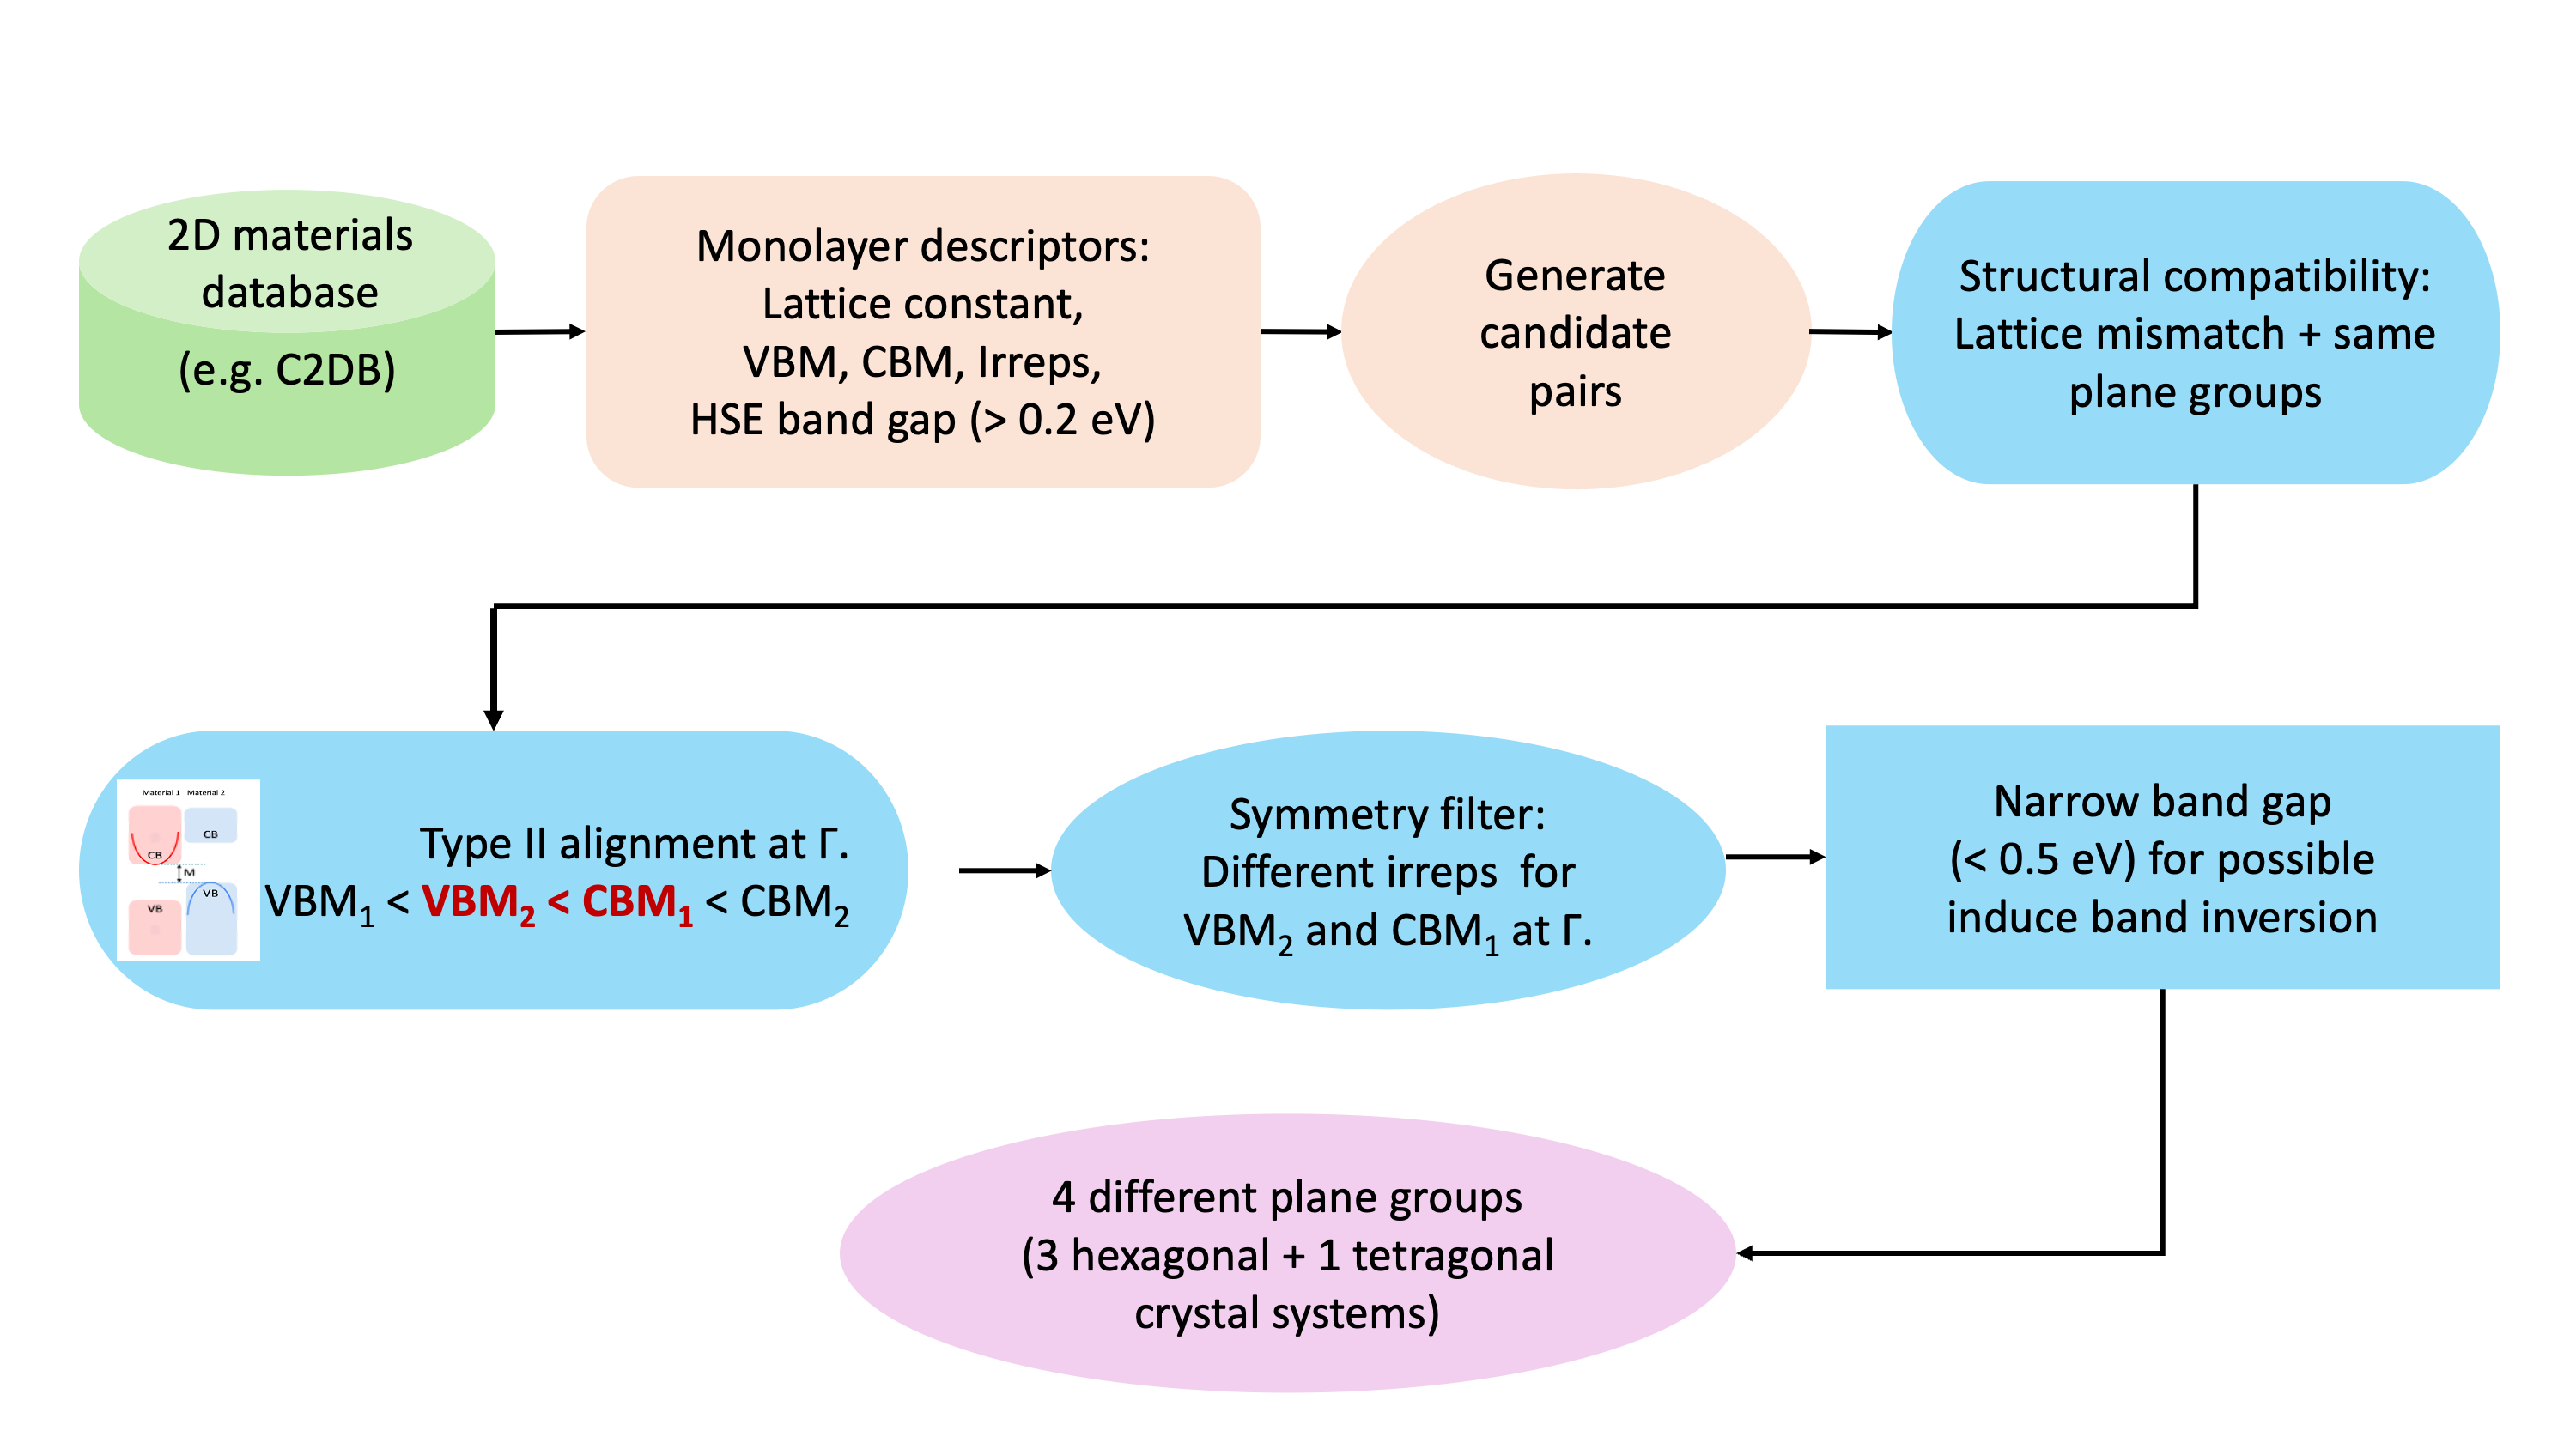
\includegraphics[width=0.9\textwidth]{images/typeII_screening_workflow2.png}}
        \put(0,82){\small\textbf{(a)}}
    \end{picture}
    \vspace{0.2em}
    % Panel (b)
    \begin{picture}(160,80)
        \put(0,0){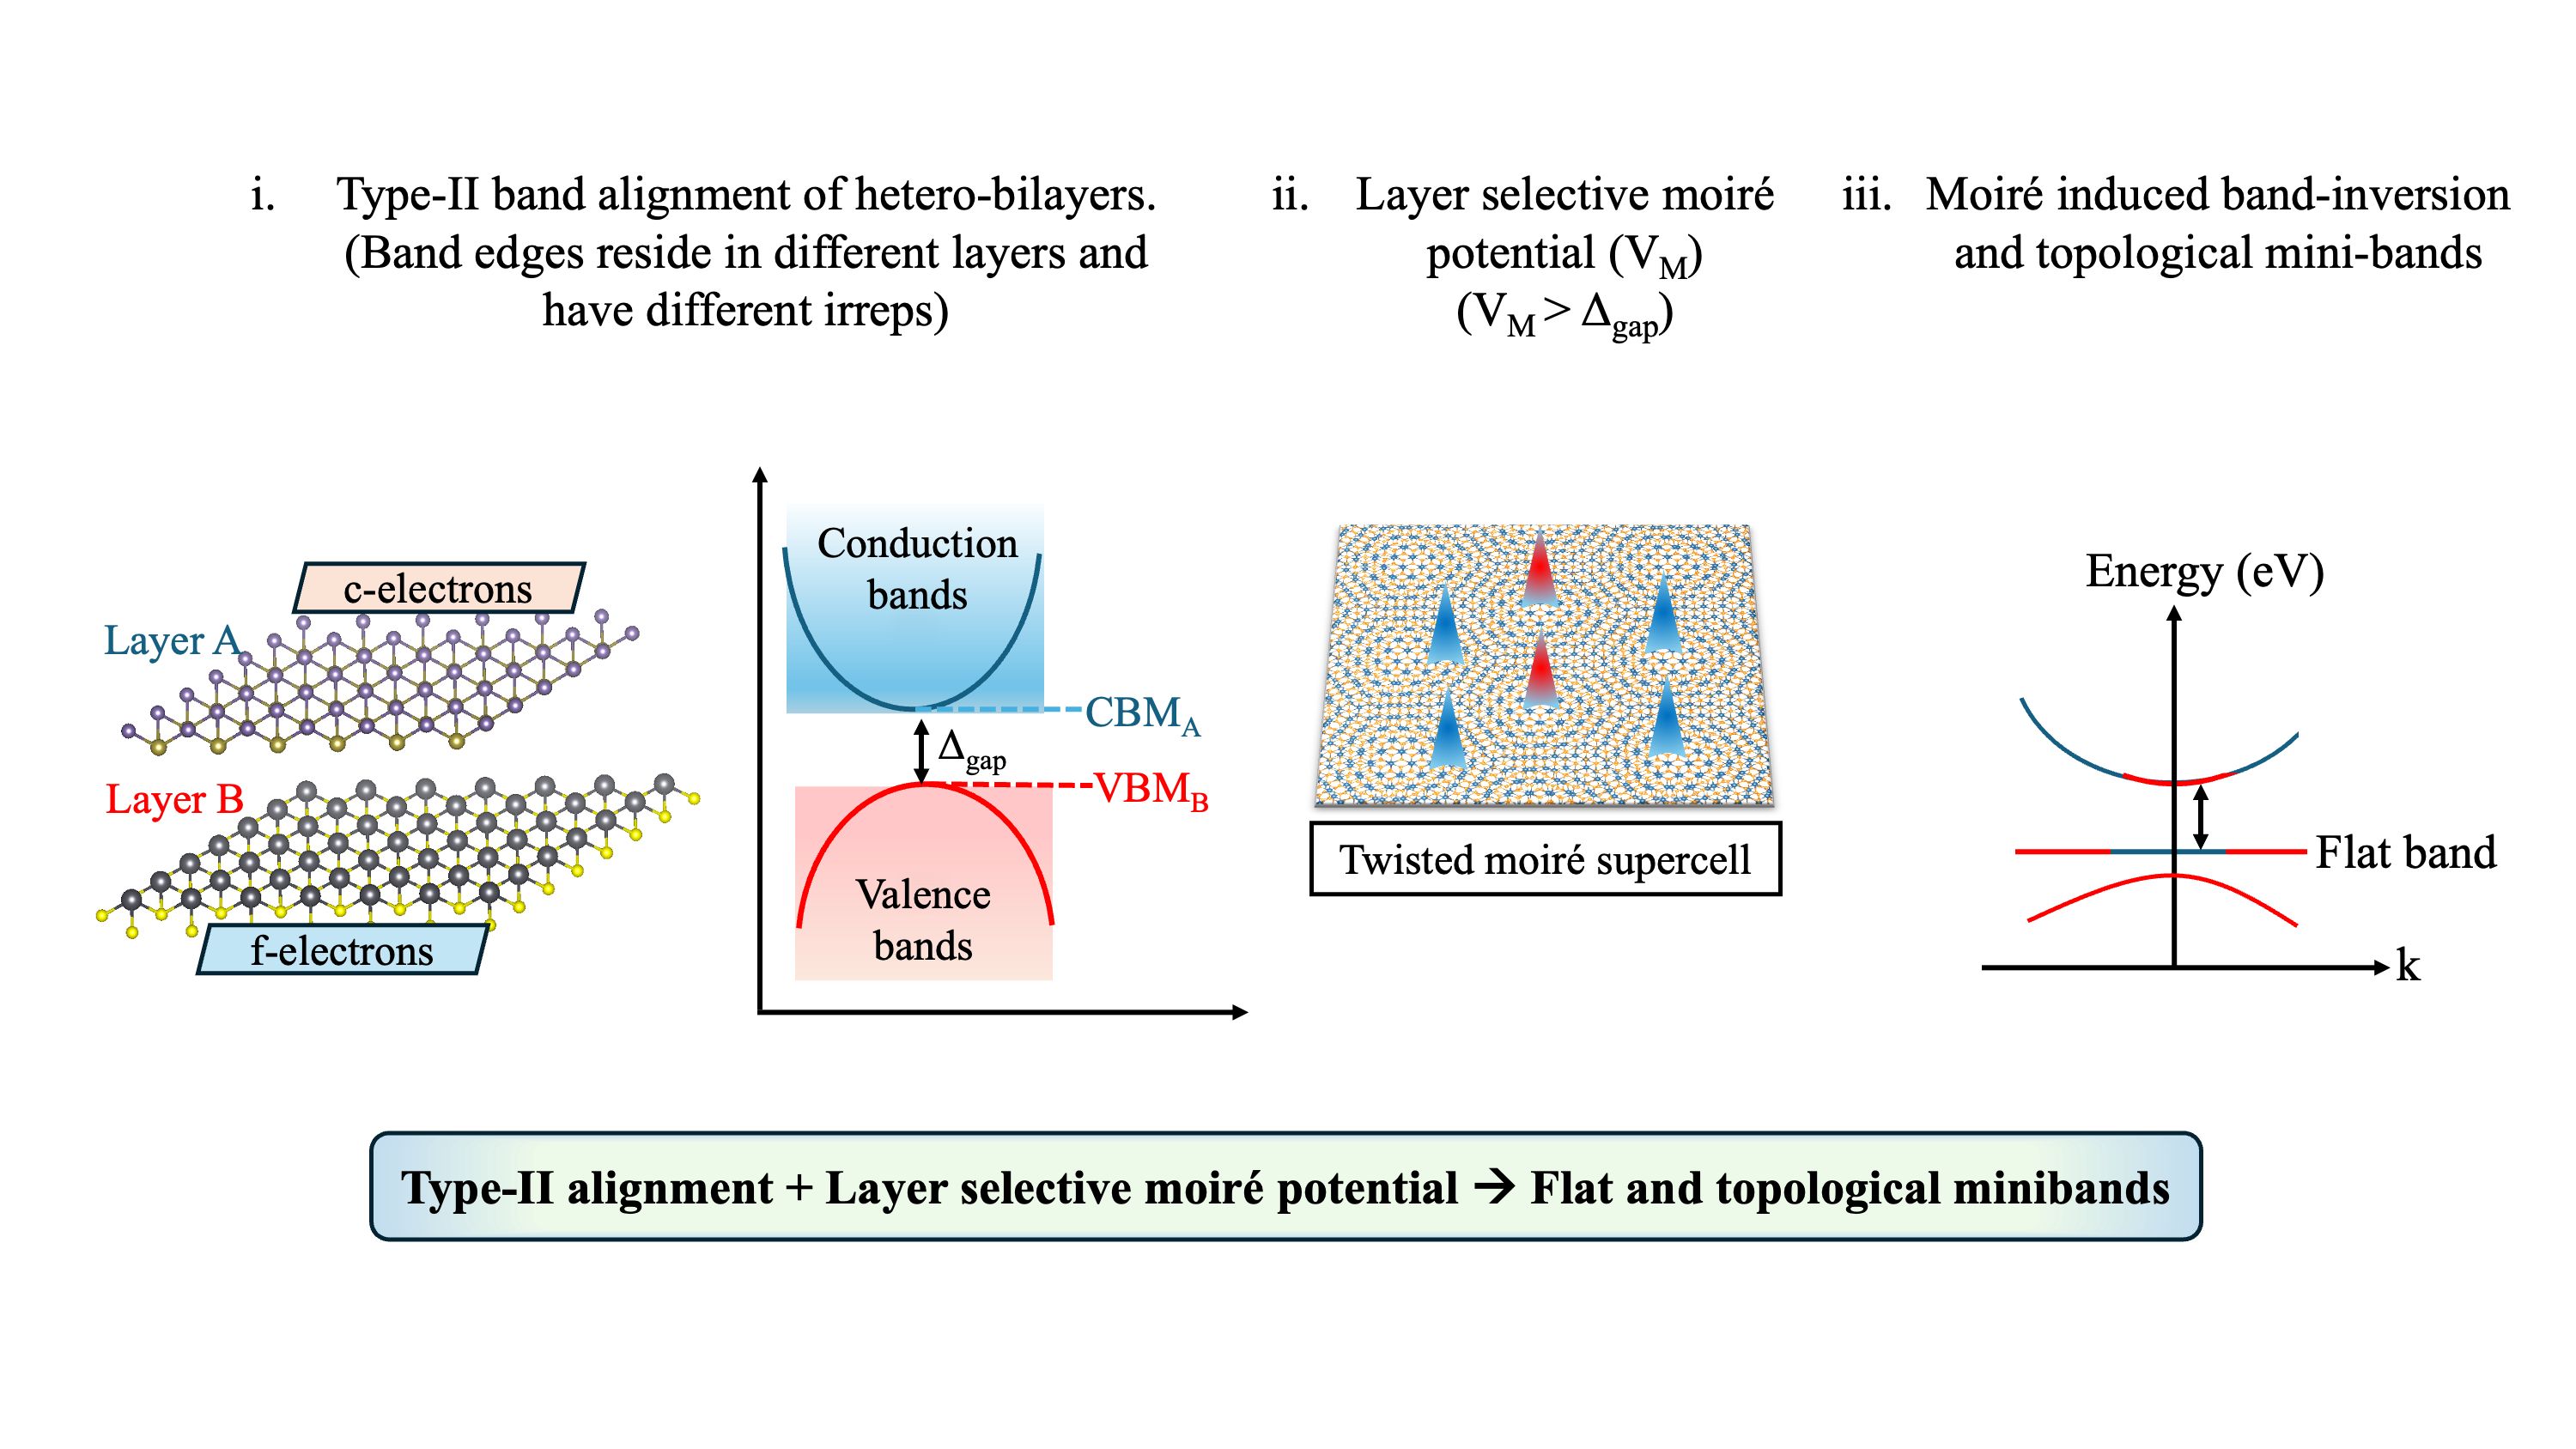
\includegraphics[width=0.9\textwidth]{images/thf_conceptual_mechanism.png}}
        \put(0,72){\small\textbf{(b)}}
    \end{picture}

    \caption{\justifying Screening workflow and type-II topological heavy-fermion design principle. (a) High-throughput screening workflow based on monolayer descriptors, type-II band alignment, symmetry filtering, and structural compatibility. (b) Schematic of the type-II THF mechanism: layer-separated conduction- and valence-band edges are driven toward inversion by a layer-selective moir\'e potential, and the resulting hybridization reconstructs the spectrum into narrow topological minibands. 
    \addCXL{In Fig. 1, I think we should emphasize the flat band gap is not directly from moire potential. In later part, we should explicitly demonstrate that. }
    }
    \label{fig:workflow_thf}
\end{figure}

The physical motivation is the type-II THF mechanism, in which the conduction and valence band edges come from different layers and are separated by a small atomic gap. A layer-selective moir\'e potential can then shift their relative energies and drive the system toward band inversion. If symmetry allows the inverted states to hybridize, the resulting gap opening provides a route to realize narrow topological minibands. The most favorable cases are those in which the relevant conduction and valence band states transform according to different irreps, ideally with angular-momentum difference $\Delta J_z=\pm 1$. Together, these filters isolate candidate type-II heterostructures whose atomic-scale electronic structure is compatible with the THF mechanism and the formation of topological minibands.

The screening workflow identifies candidate material pairs in the space groups $P\bar{3}m1$, $P\bar{6}m2$, $P\bar{4}m2$, and $P3m1$. Material pairs satisfying the screening criteria in the $P\bar{3}m1$ ($D_{3d}$) family is listed in Table~\ref{tab:p-3m1}. For each pair, we report the lattice constants, vacuum-referenced VBM and CBM energies, their irreps, the resulting type-II atomic gap, and the lattice mismatch. Candidate material pairs for the remaining symmetry families are provided in the Supporting Information. Representative heterostructures from those families are also discussed there, while the main text focuses on one representative case.

\begin{table}[htbp]
\centering
\caption{\justifying Candidate material pairs for type-II heterostructures in $P\bar{3}m1$ group, including their lattice constants, band edges (CBM/VBM) with irreducible representation (IR), type II energy gap, and lattice mismatch.}
\renewcommand{\arraystretch}{1.2}
\setlength{\tabcolsep}{5pt}
\resizebox{\textwidth}{!}{%
\begin{tabular}{c c c c c c c c}
\toprule
\textbf{Material 1} & Lattice const. (\AA) & CBM$_{M1}$ (eV) (IR) & \textbf{Material 2} & Lattice const. (\AA) & VBM$_{M2}$ (eV) (IR) & $\Delta E$ (eV) & Mismatch (\%) \\
\midrule
HgCl$_2$   & 3.994 & $-4.955$ ($\Gamma_1^+$) & PtTe$_2$     & 4.016 & $-4.966$ ($\Gamma_3^-$) & 0.011 & 0.55 \\
HgCl$_2$   & 3.994 & $-4.955$ ($\Gamma_1^+$) & Ge$_2$H$_2$   & 4.077 & $-5.337$ ($\Gamma_3^+$) & 0.382 & 2.08 \\
Tl$_2$Se$_2$ & 4.229 & $-5.433$ ($\Gamma_2^-$) & Zn$_2$Te$_2$  & 4.330 & $-5.642$ ($\Gamma_3^-$) & 0.209 & 2.39 \\
HgBr$_2$   & 4.143 & $-4.798$ ($\Gamma_1^+$) & PtTe$_2$     & 4.016 & $-4.966$ ($\Gamma_3^-$) & 0.168 & -3.07 \\
Tl$_2$S$_2$  & 4.061 & $-5.638$ ($\Gamma_2^-$) & H$_2$Si$_2$   & 3.895 & $-5.658$ ($\Gamma_3^+$) & 0.020 & -4.09 \\
Tl$_2$Se$_2$ & 4.229 & $-5.433$ ($\Gamma_2^-$) & Au$_2$I$_2$   & 4.444 & $-5.801$ ($\Gamma_3^-$) & 0.368 & 5.08 \\
Tl$_2$S$_2$  & 4.061 & $-5.638$ ($\Gamma_2^-$) & Zn$_2$Te$_2$  & 4.330 & $-5.642$ ($\Gamma_3^-$) & 0.004 & 6.62 \\
PbO$_2$    & 3.402 & $-6.939$ ($\Gamma_1^+$) & HfS$_2$      & 3.652 & $-7.048$ ($\Gamma_3^-$) & 0.109 & 7.35 \\
Tl$_2$Se$_2$ & 4.229 & $-5.433$ ($\Gamma_2^-$) & H$_2$Si$_2$   & 3.895 & $-5.658$ ($\Gamma_3^+$) & 0.225 & -7.90 \\
Tl$_2$S$_2$  & 4.061 & $-5.638$ ($\Gamma_2^-$) & PdSe$_2$     & 3.735 & $-5.960$ ($\Gamma_3^-$) & 0.322 & -8.03 \\
Tl$_2$S$_2$  & 4.061 & $-5.638$ ($\Gamma_2^-$) & Au$_2$I$_2$   & 4.444 & $-5.801$ ($\Gamma_3^-$) & 0.163 & 9.43 \\
Tl$_2$Te$_2$ & 4.520 & $-4.965$ ($\Gamma_2^-$) & Ge$_2$H$_2$   & 4.077 & $-5.337$ ($\Gamma_3^+$) & 0.372 & -9.80 \\
Tl$_2$Se$_2$ & 4.229 & $-5.433$ ($\Gamma_2^-$) & Cd$_2$Te$_2$  & 4.670 & $-5.918$ ($\Gamma_3^-$) & 0.485 & 10.43 \\
Tl$_2$Te$_2$ & 4.520 & $-4.965$ ($\Gamma_2^-$) & PtTe$_2$     & 4.016 & $-4.966$ ($\Gamma_3^-$) & 0.001 & -11.15 \\
Tl$_2$S$_2$  & 4.061 & $-5.638$ ($\Gamma_2^-$) & Ag$_2$I$_2$   & 4.577 & $-6.116$ ($\Gamma_3^-$) & 0.478 & 12.71 \\
Tl$_2$S$_2$  & 4.061 & $-5.638$ ($\Gamma_2^-$) & Cd$_2$Te$_2$  & 4.670 & $-5.918$ ($\Gamma_3^-$) & 0.280 & 15.00 \\
PbO$_2$    & 3.402 & $-6.939$ ($\Gamma_1^+$) & Zn$_2$S$_2$   & 3.923 & $-7.041$ ($\Gamma_3^-$) & 0.102 & 15.31 \\
HgCl$_2$   & 3.994 & $-4.955$ ($\Gamma_1^+$) & Zr$_2$CO$_2$  & 3.300 & $-5.103$ ($\Gamma_3^-$) & 0.148 & -17.38 \\
HgCl$_2$   & 3.994 & $-4.955$ ($\Gamma_1^+$) & Sc$_2$CF$_2$  & 3.267 & $-5.443$ ($\Gamma_3^-$) & 0.488 & -18.20 \\
Tl$_2$S$_2$  & 4.061 & $-5.638$ ($\Gamma_2^-$) & Hf$_2$CO$_2$  & 3.277 & $-5.870$ ($\Gamma_3^-$) & 0.232 & -19.31 \\
HgBr$_2$   & 4.143 & $-4.798$ ($\Gamma_1^+$) & Zr$_2$CO$_2$  & 3.300 & $-5.103$ ($\Gamma_3^-$) & 0.305 & -20.35 \\
Tl$_2$Se$_2$ & 4.229 & $-5.433$ ($\Gamma_2^-$) & Hf$_2$CO$_2$  & 3.277 & $-5.870$ ($\Gamma_3^-$) & 0.437 & -22.51 \\
Tl$_2$Se$_2$ & 4.229 & $-5.433$ ($\Gamma_2^-$) & Sc$_2$CF$_2$  & 3.267 & $-5.443$ ($\Gamma_3^-$) & 0.010 & -22.75 \\
PbO$_2$    & 3.402 & $-6.939$ ($\Gamma_1^+$) & MgI$_2$      & 4.207 & $-7.173$ ($\Gamma_3^-$) & 0.234 & 23.66 \\
\bottomrule
\end{tabular}%
}
\label{tab:p-3m1}
\end{table}

The screened candidates are then studied through a sequence of first-principles calculations. Monolayer band structures are first computed without SOC, and the $\Gamma$-point irreps of the band-edge states are identified. SOC is then included to obtain the corresponding double-group irreps \cite{Iraola2022IrRep}. A commensurate bilayer is constructed at a common in-plane lattice constant, the atomic positions are relaxed, and the band structure of the relaxed heterostructure is evaluated with SOC and layer projections. This procedure tracks the evolution of band alignment, symmetry labels, and layer character from isolated monolayers to the bilayer, and shows that the resulting low-energy electronic structure remains consistent with the type-II THF picture.

We discuss HgCl$_2$/PtTe$_2$ as a representative example from the space group $P\bar{3}m1$, and representatives from other space groups are discussed in the SI. The isolated monolayers show the desired type-II alignment: the conduction-band minimum comes from HgCl$_2$, whereas the valence-band maximum is provided by PtTe$_2$. At $\Gamma$, the HgCl$_2$ conduction edge transforms as $\Gamma_1^+$ and the PtTe$_2$ valence edge as $\Gamma_3^-$. The atomic offset gap between these states is about $0.01$~eV, placing the system in the narrow-gap regime relevant to moir\'e potential induced band inversion. With SOC included at the r2SCAN level~\cite{furness2020accurate}, the HgCl$_2$ conduction edge becomes $\bar{\Gamma}_6^+$, while the PtTe$_2$ valence edge splits into the degenerate doublet $\bar{\Gamma}_4^- \bar{\Gamma}_5^-$. The monolayer analysis, therefore, indicates type-II alignment, a very small atomic gap, and symmetry at $\Gamma$ compatible with interband coupling.

The HgCl$_2$/PtTe$_2$ bilayer is then constructed and relaxed to determine whether these features persist after stacking. In the commensurate heterostructure calculation, HgCl$_2$ is strained to the PtTe$_2$ lattice constant. The stacked geometry breaks inversion symmetry and lowers the point group from $D_{3d}$ for the isolated monolayers to $C_{3v}$ for the bilayer. The relaxed r2SCAN+SOC band structure preserves the type-II ordering and shows a band gap of $0.12$~eV at $\Gamma$. Layer projected bandstructure shows that the VBM remains localized on PtTe$_2$ and transforms as $\bar{\Gamma}_5\bar{\Gamma}_6$ with $J_z=\pm 3/2$, whereas the HgCl$_2$-derived CBM transforms as $\bar{\Gamma}_4$ with $J_z=\pm 1/2$ as shown in (Fig.~\ref{fig:hgcl2_ptte2}). 

\begin{figure}[htbp]
 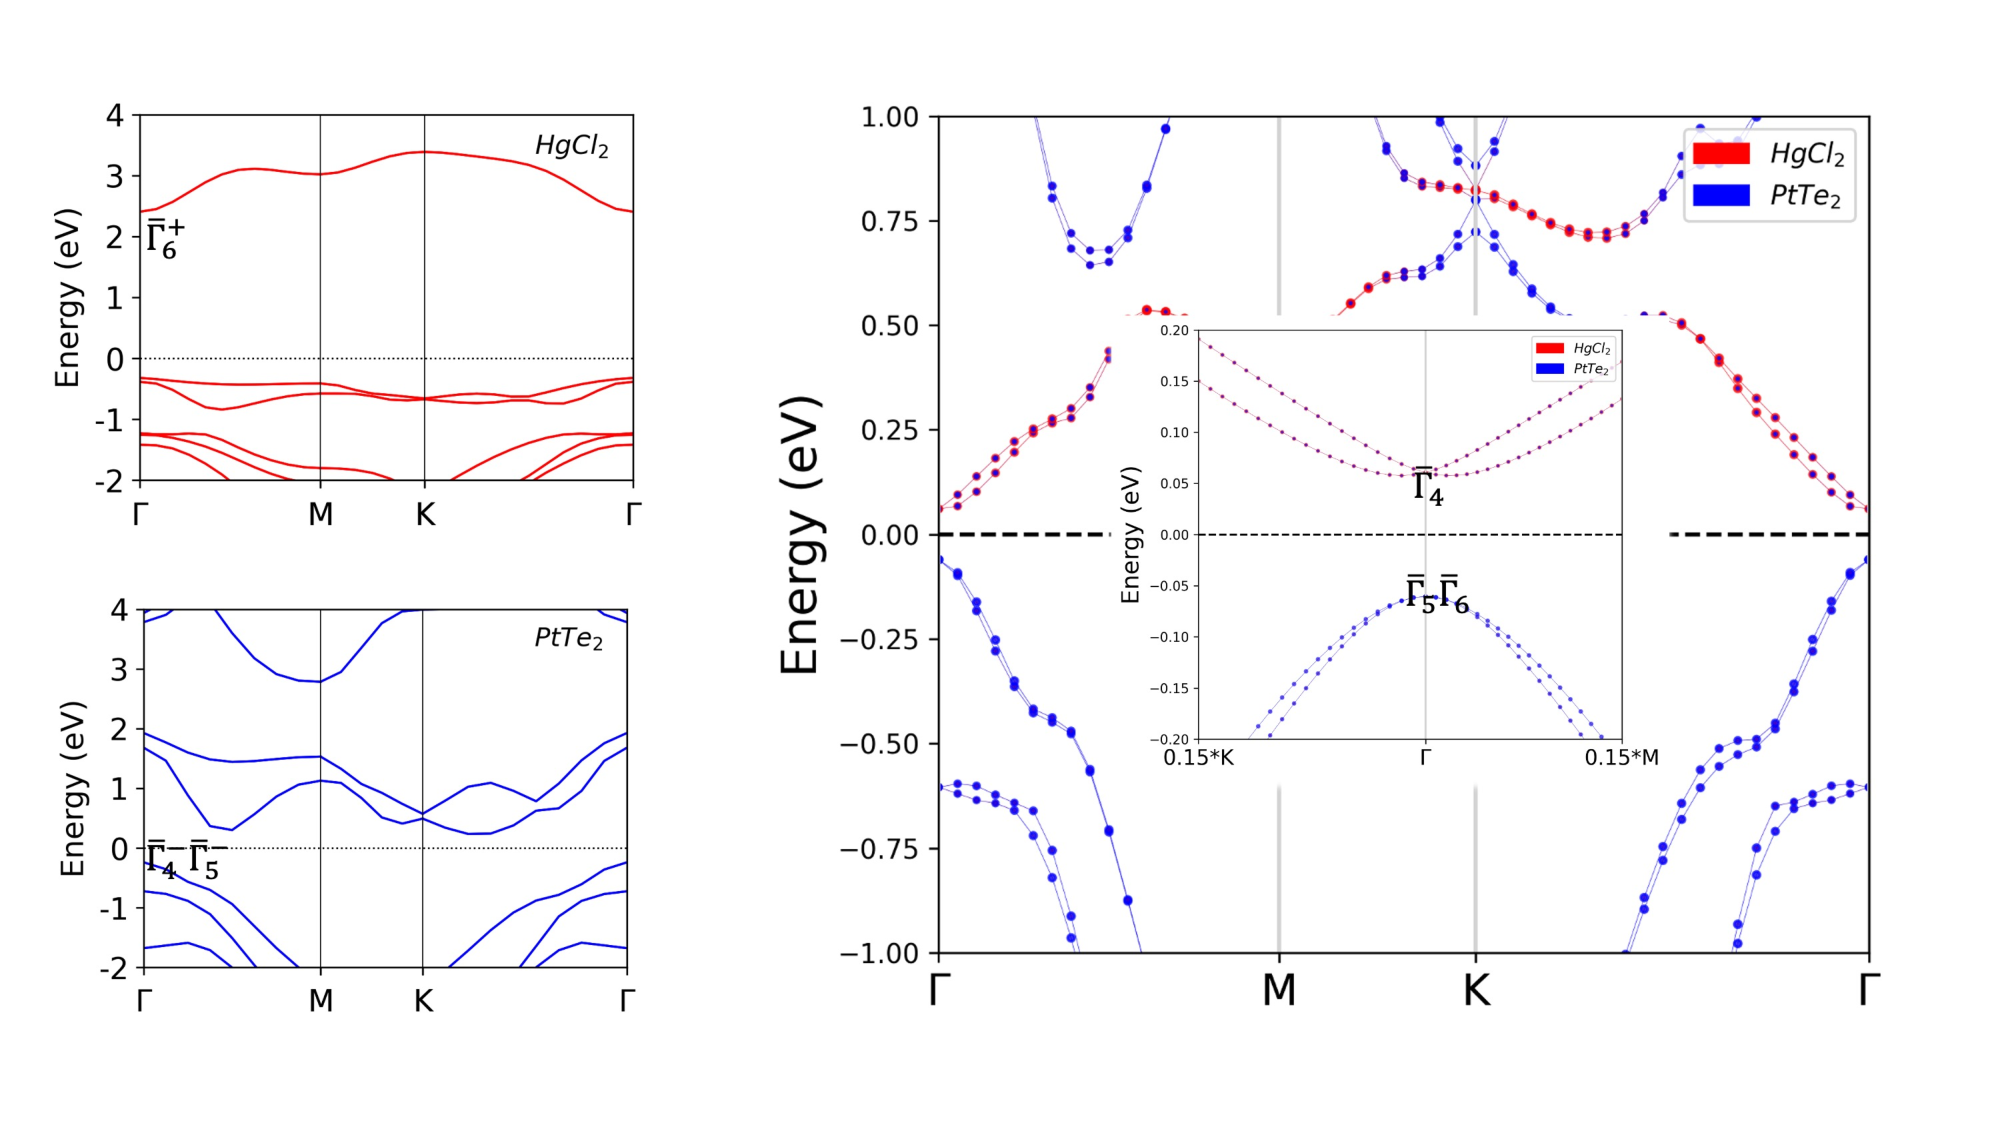
\includegraphics[width=1.0\textwidth]{images/hgcl2_ptte2_bands_layer_resolved.pdf}
 \caption{\justifying Layer-resolved band structure of HgCl$_2$/PtTe$_2$ including SOC. A type-II direct gap is observed at $\Gamma$, with the valence-band maximum on PtTe$_2$ and the conduction-band minimum on HgCl$_2$. The inset shows a zoomed view near $\Gamma$ using DFT calculations, confirming the atomic gap.}
 \label{fig:hgcl2_ptte2}
\end{figure}

These results show HgCl$_2$/PtTe$_2$ as a suitable candidate for the type-II THF mechanism. The relaxed bilayer preserves the type-II alignment with band edges from two different layers and the direct band gap at $\Gamma$ is small. At the same time, the angular-momentum difference between the conduction and valence-band states is $\Delta J_z=\pm 1$. This is the structure required for a BHZ-like low-energy Hamiltonian. HgCl$_2$/PtTe$_2$ therefore provides a realistic atomic-scale starting point for moir\'e-potential-induced band inversion and the formation of topological minibands. Representative examples from the remaining symmetry families are presented in the Supporting Information.

The little group at $\Gamma$ is $D_{3d}$ in space group $P\bar{3}m1$ which is reduced to $C_{3v}$ in the heterostructure. The character tables for these two groups are shown in SI. When the SOC is not included, the $\mathbf{\Gamma}^+_1$ and $\mathbf{\Gamma}^-_3$ irreps of the $D_{3d}$ group for the conduction of HgCl$_2$ and the valence band of PtTe$_2$ correspond to the $\mathbf{\Gamma}_1$ and $\mathbf{\Gamma}_3$ irreps in the $C_{3v}$ group. When the SOC is included,  the irreps of conduction and valence bands are $\bar{\Gamma}_4$ and $\bar{\Gamma}_5\bar{\Gamma}_6$, respectively. The conduction bands exhibit Rashba SOC just as in the case of Tl$_2$Se$_2$/Zn$_2$Te$_2$ heterostructure discussed in Ref.\cite{Liu2025IdealTHF}. The effective model is given by
\begin{eqnarray}
&&H_{\mathrm{hetero}}(\kk)=
\begin{pmatrix}
H^{\uparrow\uparrow}_{\mathrm{hetero}}(\kk) & H^{\uparrow\downarrow}_{\mathrm{hetero}}(\kk) \\
\bigl(H^{\uparrow\downarrow}_{\mathrm{hetero}}(\kk)\bigr)^\dagger & H^{\downarrow\downarrow}_{\mathrm{hetero}}(\kk)
\end{pmatrix},\nonumber\\
&&H^{\uparrow\uparrow}_{\mathrm{hetero}}(\kk)=
\begin{pmatrix}
E_1 + A_1 k^2 & i B_0 (k_x + i k_y) \nonumber \\
- i B_0 (k_x - i k_y) & E_2 + A_2 k^2
\end{pmatrix}, H^{\downarrow\downarrow}_{\mathrm{hetero}}(\kk)=
\bigl(H^{\uparrow\uparrow}_{\mathrm{hetero}}(-\kk)\bigr)^*, \\
&&H^{\uparrow\downarrow}_{\mathrm{hetero}}(\kk)=
\begin{pmatrix}
- i R_0 k_- & 0 \\
0 & 0
\end{pmatrix}. \label{Eq;Rashba}
\end{eqnarray}

\begin{figure}[htbp]
 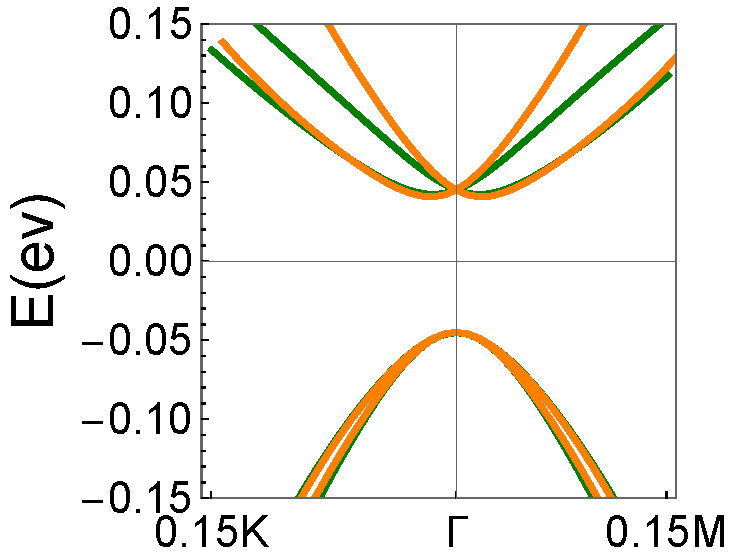
\includegraphics[width=0.5\textwidth]{images/fit_p-3m1.pdf}
 \caption{\justifying  A zoomed-in view of the band dispersion near $\mathbf{\Gamma}$ point from DFT calculation (green curves) and the corresponding effective model fitting (orange curves).}
 \label{fig:fit_p-3m1}
\end{figure}
By choosing the parameters $E_1=-E_2=0.045$~eV, $A_1=0.289~a_0^2\!\cdot\!\mathrm{eV}$, $B_0=0.257~a_0\!\cdot\!\mathrm{eV}$, $A_2=-0.434~a_0^2\!\cdot\!\mathrm{eV}$, and $R_0=0.134~a_0\!\cdot\!\mathrm{eV}$, we obtain the band dispersions from the effective model, shown as the orange curves in Fig.~\ref{fig:fit_p-3m1}. The effective model captures the low-energy band dispersions of the heterostructure well. 

% Add discussion on origin of topological miniband

\subsection{Moir\'e potential} %add discussion on moire potential here

We next consider the introduction of a moir\'e potential in one layer of the heterostructure. Although this can in principle be obtained from direct DFT calculations on twisted moir\'e supercells, the required system sizes are computationally demanding. We therefore use a machine-learned interatomic potential within the NequIP framework \cite{Batzner2022NequIP}, trained on energies and forces from VASP machine-learning force field (MLFF) calculations for locally shifted bilayer configurations of \ce{PtTe2}. The trained model enables efficient relaxation of the twisted moir\'e supercells, and self-consistent VASP calculations on the relaxed structures are then used to extract the moir\'e potential from the electronic potential profile. 

Fig.~\ref{fig:potential_dft} shows the electrostatic potential modulation in the twisted \ce{PtTe2} bilayer. 
The potentials are evaluated on planes located a distance $d=3~\text{\AA}$ away from the average topmost and bottommost atomic layers. 
The top and bottom potential maps show a spatially varying superlattice modulation that follows the moir\'e reconstruction. 
Their difference, $\Delta V(\mathbf{r}) =
V_{\mathrm{top}}(\mathbf{r}) - V_{\mathrm{bot}}(\mathbf{r})$ , captures the layer-asymmetric component of the electrostatic potential.
The potential variation decreases gradually as the sampling plane is moved away from the bilayer toward the vacuum region. 
Near the relaxed interlayer distance, $d_{\mathrm{int}}=2.95~\text{\AA}$, the potential lies in the weakly varying part of the distance-dependent curve. This indicates that the strongest electrostatic modulation is localized near the atomic layers and decays away from the bilayer. Such a spatially varying potential provides the microscopic origin of the moir\'e potential used in the effective model and can modify the layer-resolved band-edges. 

The \ce{PtTe2} calculation is used here as a representative estimate of the moir\'e electrostatic potential. From the maps at \(d=3~\text{\AA}\), \(V_{\mathrm{top}}\) and \(V_{\mathrm{bot}}\) vary by approximately \(-70\) to \(+70~\mathrm{meV}\), while the layer-asymmetric component \(\Delta V(\mathbf{r})\) is nearly \(-25\) to \(+25~\mathrm{meV}\). This gives a peak-to-peak layer-dependent modulation of about \(50~\mathrm{meV}\), comparable to the \(\sim 40~\mathrm{meV}\) scale required in the Tl$_2$Se$_2$/Zn$_2$Te$_2$ effective model. In principle, such an externally supplied moir\'e potential could be applied to the candidate type-II heterostructures identified in this family, provided that the potential-generating layer does not introduce low-energy bands that strongly hybridize with the active band-edge states. 
\begin{comment}
\begin{figure}[htbp]
    \centering

    \begin{subfigure}{0.48\textwidth}
        \centering
        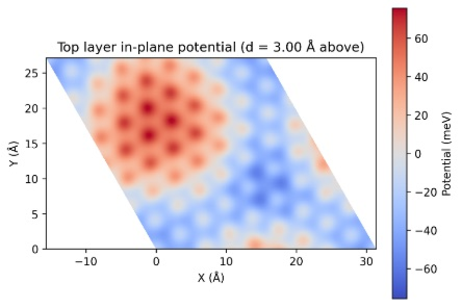
\includegraphics[width=\textwidth]{images/top.pdf}
        \caption{$V_{\mathrm{top}}(\mathbf{r})$}
        \label{fig:potential_dft_top}
    \end{subfigure}
    \hfill
    \begin{subfigure}{0.48\textwidth}
        \centering
        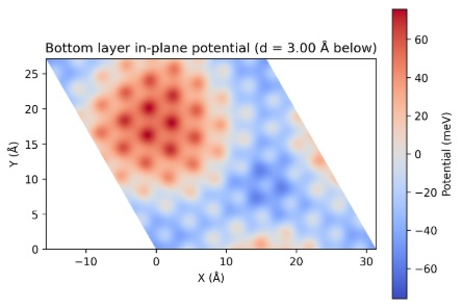
\includegraphics[width=\textwidth]{images/bottom.pdf}
        \caption{$V_{\mathrm{bot}}(\mathbf{r})$}
        \label{fig:potential_dft_bottom}
    \end{subfigure}

    \vspace{0.5em}

    \begin{subfigure}{0.48\textwidth}
        \centering
        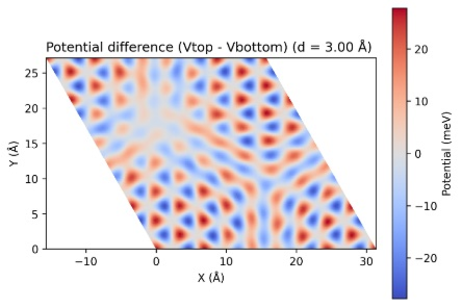
\includegraphics[width=\textwidth]{images/difference.pdf}
        \caption{$\Delta V(\mathbf{r})=V_{\mathrm{top}}(\mathbf{r})-V_{\mathrm{bot}}(\mathbf{r})$}
        \label{fig:potential_dft_difference}
    \end{subfigure}
    \hfill
    \begin{subfigure}{0.48\textwidth}
        \centering
        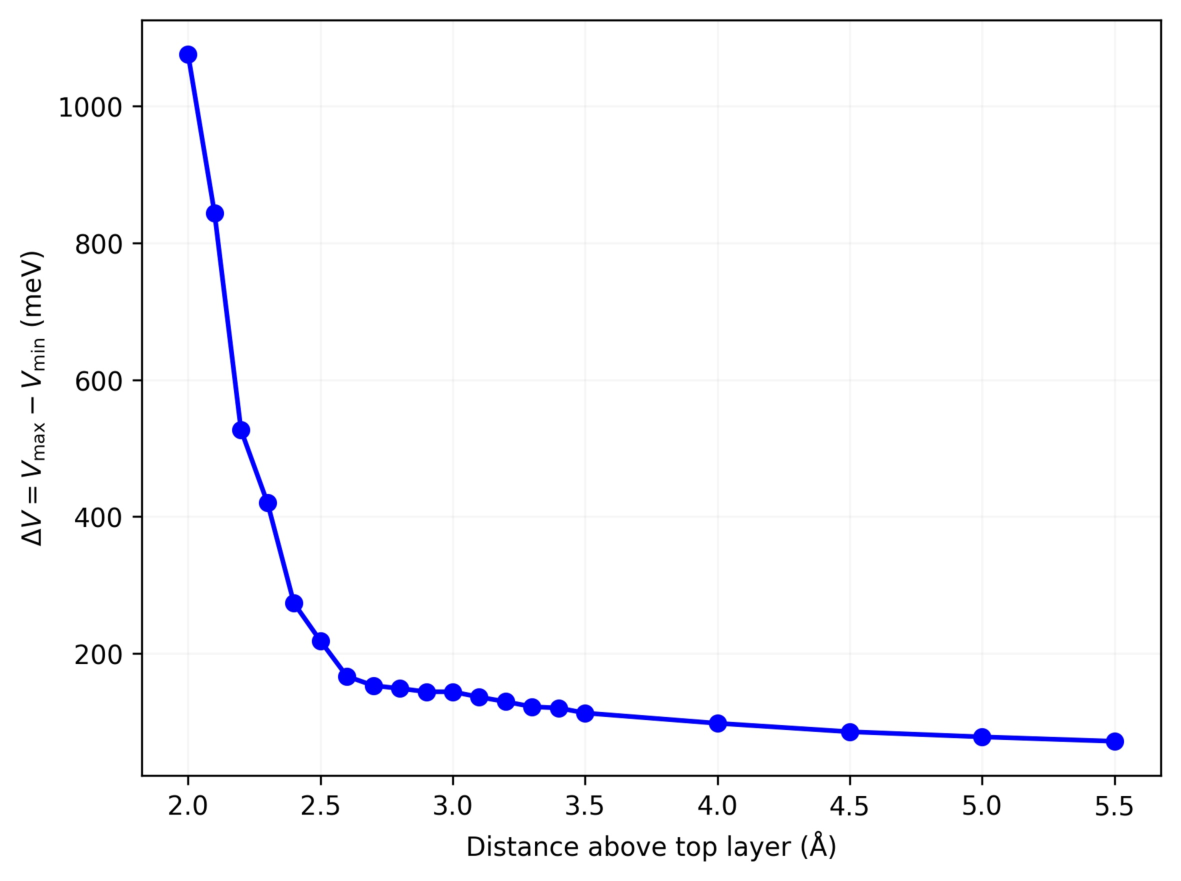
\includegraphics[width=\textwidth]{images/potential_variation.pdf}
        \caption{Potential variation with sampling distance}
        \label{fig:potential_dft_spacing}
    \end{subfigure}

    \caption{Electrostatic superlattice potential of twisted \ce{PtTe2} at a twist angle of \(7.34^\circ\). 
    (a,b) Electrostatic potential sampled on planes located \(d=3~\text{\AA}\) away from the average top and bottom outermost Te layers, respectively. 
    (c) Layer-asymmetric potential difference, \(\Delta V(\mathbf{r})=V_{\mathrm{top}}(\mathbf{r})-V_{\mathrm{bot}}(\mathbf{r})\), showing the spatial modulation of the electrostatic potential across the moir\'e supercell. 
    (d) Variation of the electrostatic potential as a function of sampling distance from the top Te layer.}
    \label{fig:potential_dft}
\end{figure}
\end{comment}
\section{Methods}

\subsection{DFT calculations}
The electronic structures of monolayers, together with their heterostructure, were calculated using VASP~\cite{kresse1996efficiency}. Vacuum-aligned band-edge energies for screening were obtained with the HSE06 hybrid functional~\cite{heyd2003hybrid}, while the further analysis of selected monolayers and heterostructures, including SOC, was performed using the r$^2$SCAN meta-GGA functional~\cite{furness2020accurate}. Atomic positions were relaxed until the residual forces were below 0.02~eV/\AA, with the electronic convergence threshold set to $10^{-7}$~eV. A vacuum spacing of about 15~\AA\ was applied along the out-of-plane direction. SOC was included self-consistently in the final band-structure calculations. The irreps of the band-edge states were then determined at the high-symmetry momenta using post-processing tools such as \texttt{Irvsp}~\cite{Gao2021Irvsp} or \texttt{IrRep} \cite{Iraola2022IrRep}. 

\subsection{Topological heavy fermion model}
\noindent The low-energy bands near $\Gamma$ can be described by a BHZ-type Hamiltonian together with a moir\'e potential \cite{Bernevig2006QSH, Liu2025IdealTHF},
\begin{equation}
\hat{H} = \hat{H}_{\rm BHZ} + \hat{H}_M .
\end{equation}
The BHZ Hamiltonian is given by
\begin{equation}
\hat{H}_{\rm BHZ}(\mathbf{k}) =
\begin{pmatrix}
\epsilon(\mathbf{k}) + M(\mathbf{k}) & A k_+ \\
A k_- & \epsilon(\mathbf{k}) - M(\mathbf{k})
\end{pmatrix},
\label{eq:BHZ}
\end{equation}
where
\begin{align}
\epsilon(\mathbf{k}) &= D k^2 , \\
M(\mathbf{k}) &= m + B k^2 , \\
k_\pm &= k_x \pm i k_y .
\end{align}
Here $\epsilon(\mathbf{k})$ represents an overall energy shift that does not affect the band topology, while the mass term $M(\mathbf{k})$ controls the band inversion and thus the topological character of the system. The linear terms $A k_\pm$ describe Dirac-like coupling between the conduction and the valence bands. In the strong moir\'e modulation limit, this description can be further reduced to a minimal THF model consisting of a dispersive $c$-like band coupled to a localized moir\'e bound state derived from the valence sector, with symmetry-constrained hybridization \cite{Liu2025IdealTHF}.

\subsection{Estimation of moir\'e potential}
The moir\'e potential is estimated from the variation of bilayer energy with local stacking. For this, we first create a 2x2 supercell, generate a set of laterally shifted bilayer configurations, and relax them. We then perform VASP MLFF calculations for that set of shifted bilayer configurations, which are computationally efficient and thereby reduce training time during the simulation loop. The resulting energies and forces are used to build a training set for the machine learning force field based on an E(3)-equivariant graph neural network (NequIP) ~\cite{Batzner2022NequIP}. The trained model is then used to relax the twisted moir\'e supercells using ASE. Self-consistent VASP calculations are carried out for the relaxed moir\'e structures, and the moir\'e potential is extracted from the spatial variation of the electronic potential.

\section*{References}
\bibliographystyle{apsrev4-2}
\bibliography{references.bib}
\end{document}